\chapter{Generation of Seed Light}\label{generationOfSeedLight}

In this chapter, we will discuss the design and construction of the Master Laser. 

\section{Stabilization of Master Laser}
\subsection{Master Laser Layout}
The master laser is a 408 nm extended cavity diode laser(ECDL). It consists of a laser diode mounted in a temperature-controlled housing from the Thorlabs LDM21 family of products. It is collimated by a small, aspherical lens (Thorlabs C570TM-A). A picture of the maseter laser can be seen in Fig.\,\ref{master_laser_photo}.

\begin{figure}
\centerline{
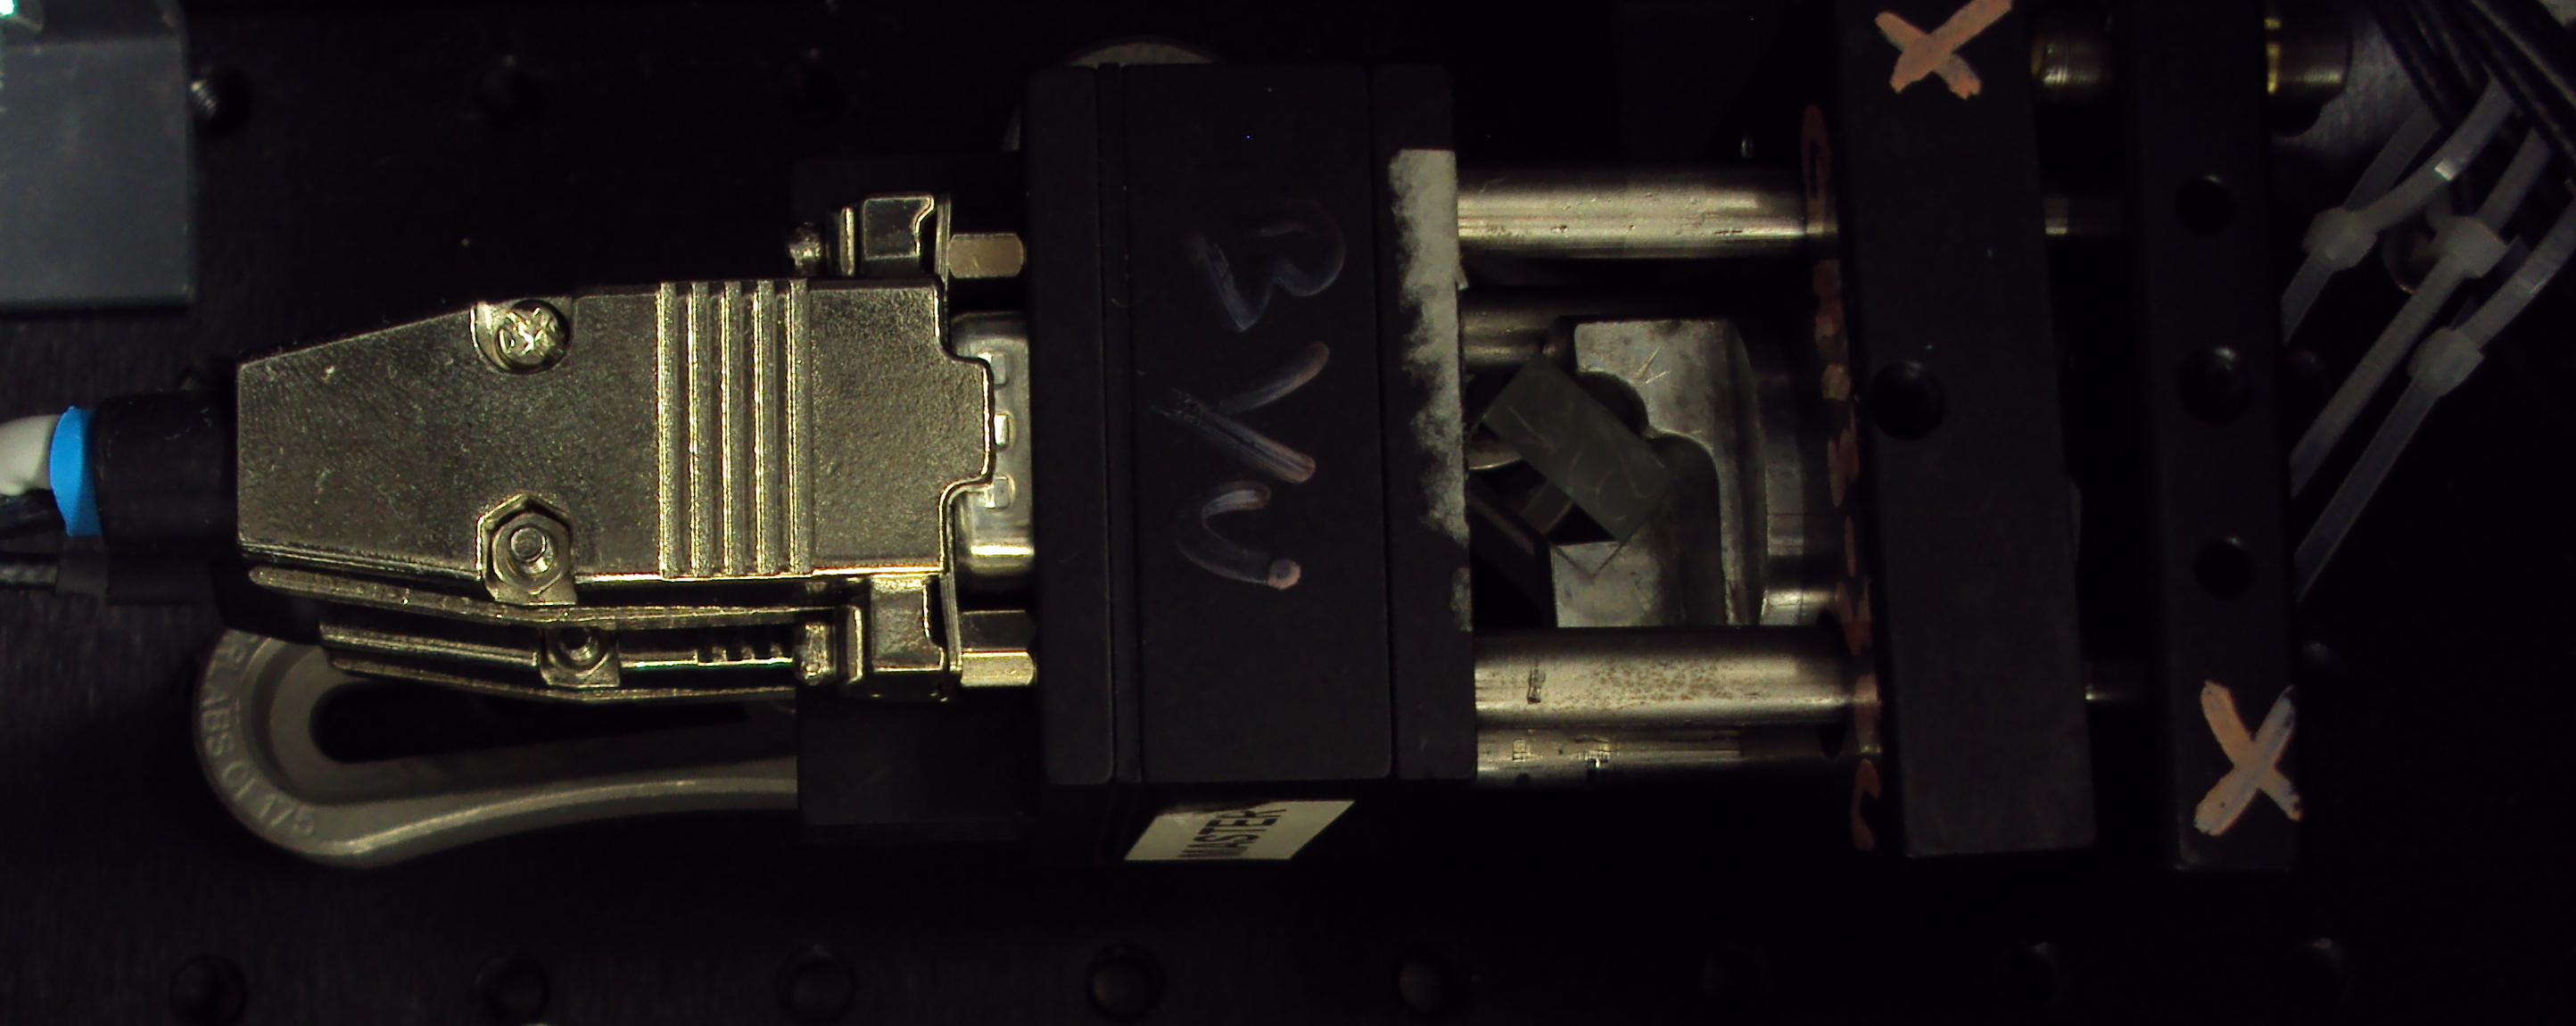
\includegraphics[width=0.95\textwidth]{master_laser.JPG}}
\caption[Photograph of Master Laser]{\label{master_laser_photo} The master laser is housed in the black box in the upper right of the picture. The diffraction grating that is used for feedback is mounted on a custom mount close to the master laser aperture. We initially tried several other configurations. However, after several iterations, we found that the use of the metal rods to directly mechanically couple the laser and grating were necessary for stable single-mode operation. We also found through trial and error that the distance of $\sim$2 cm seemed to work. }
\end{figure}

\begin{figure}
\centerline{
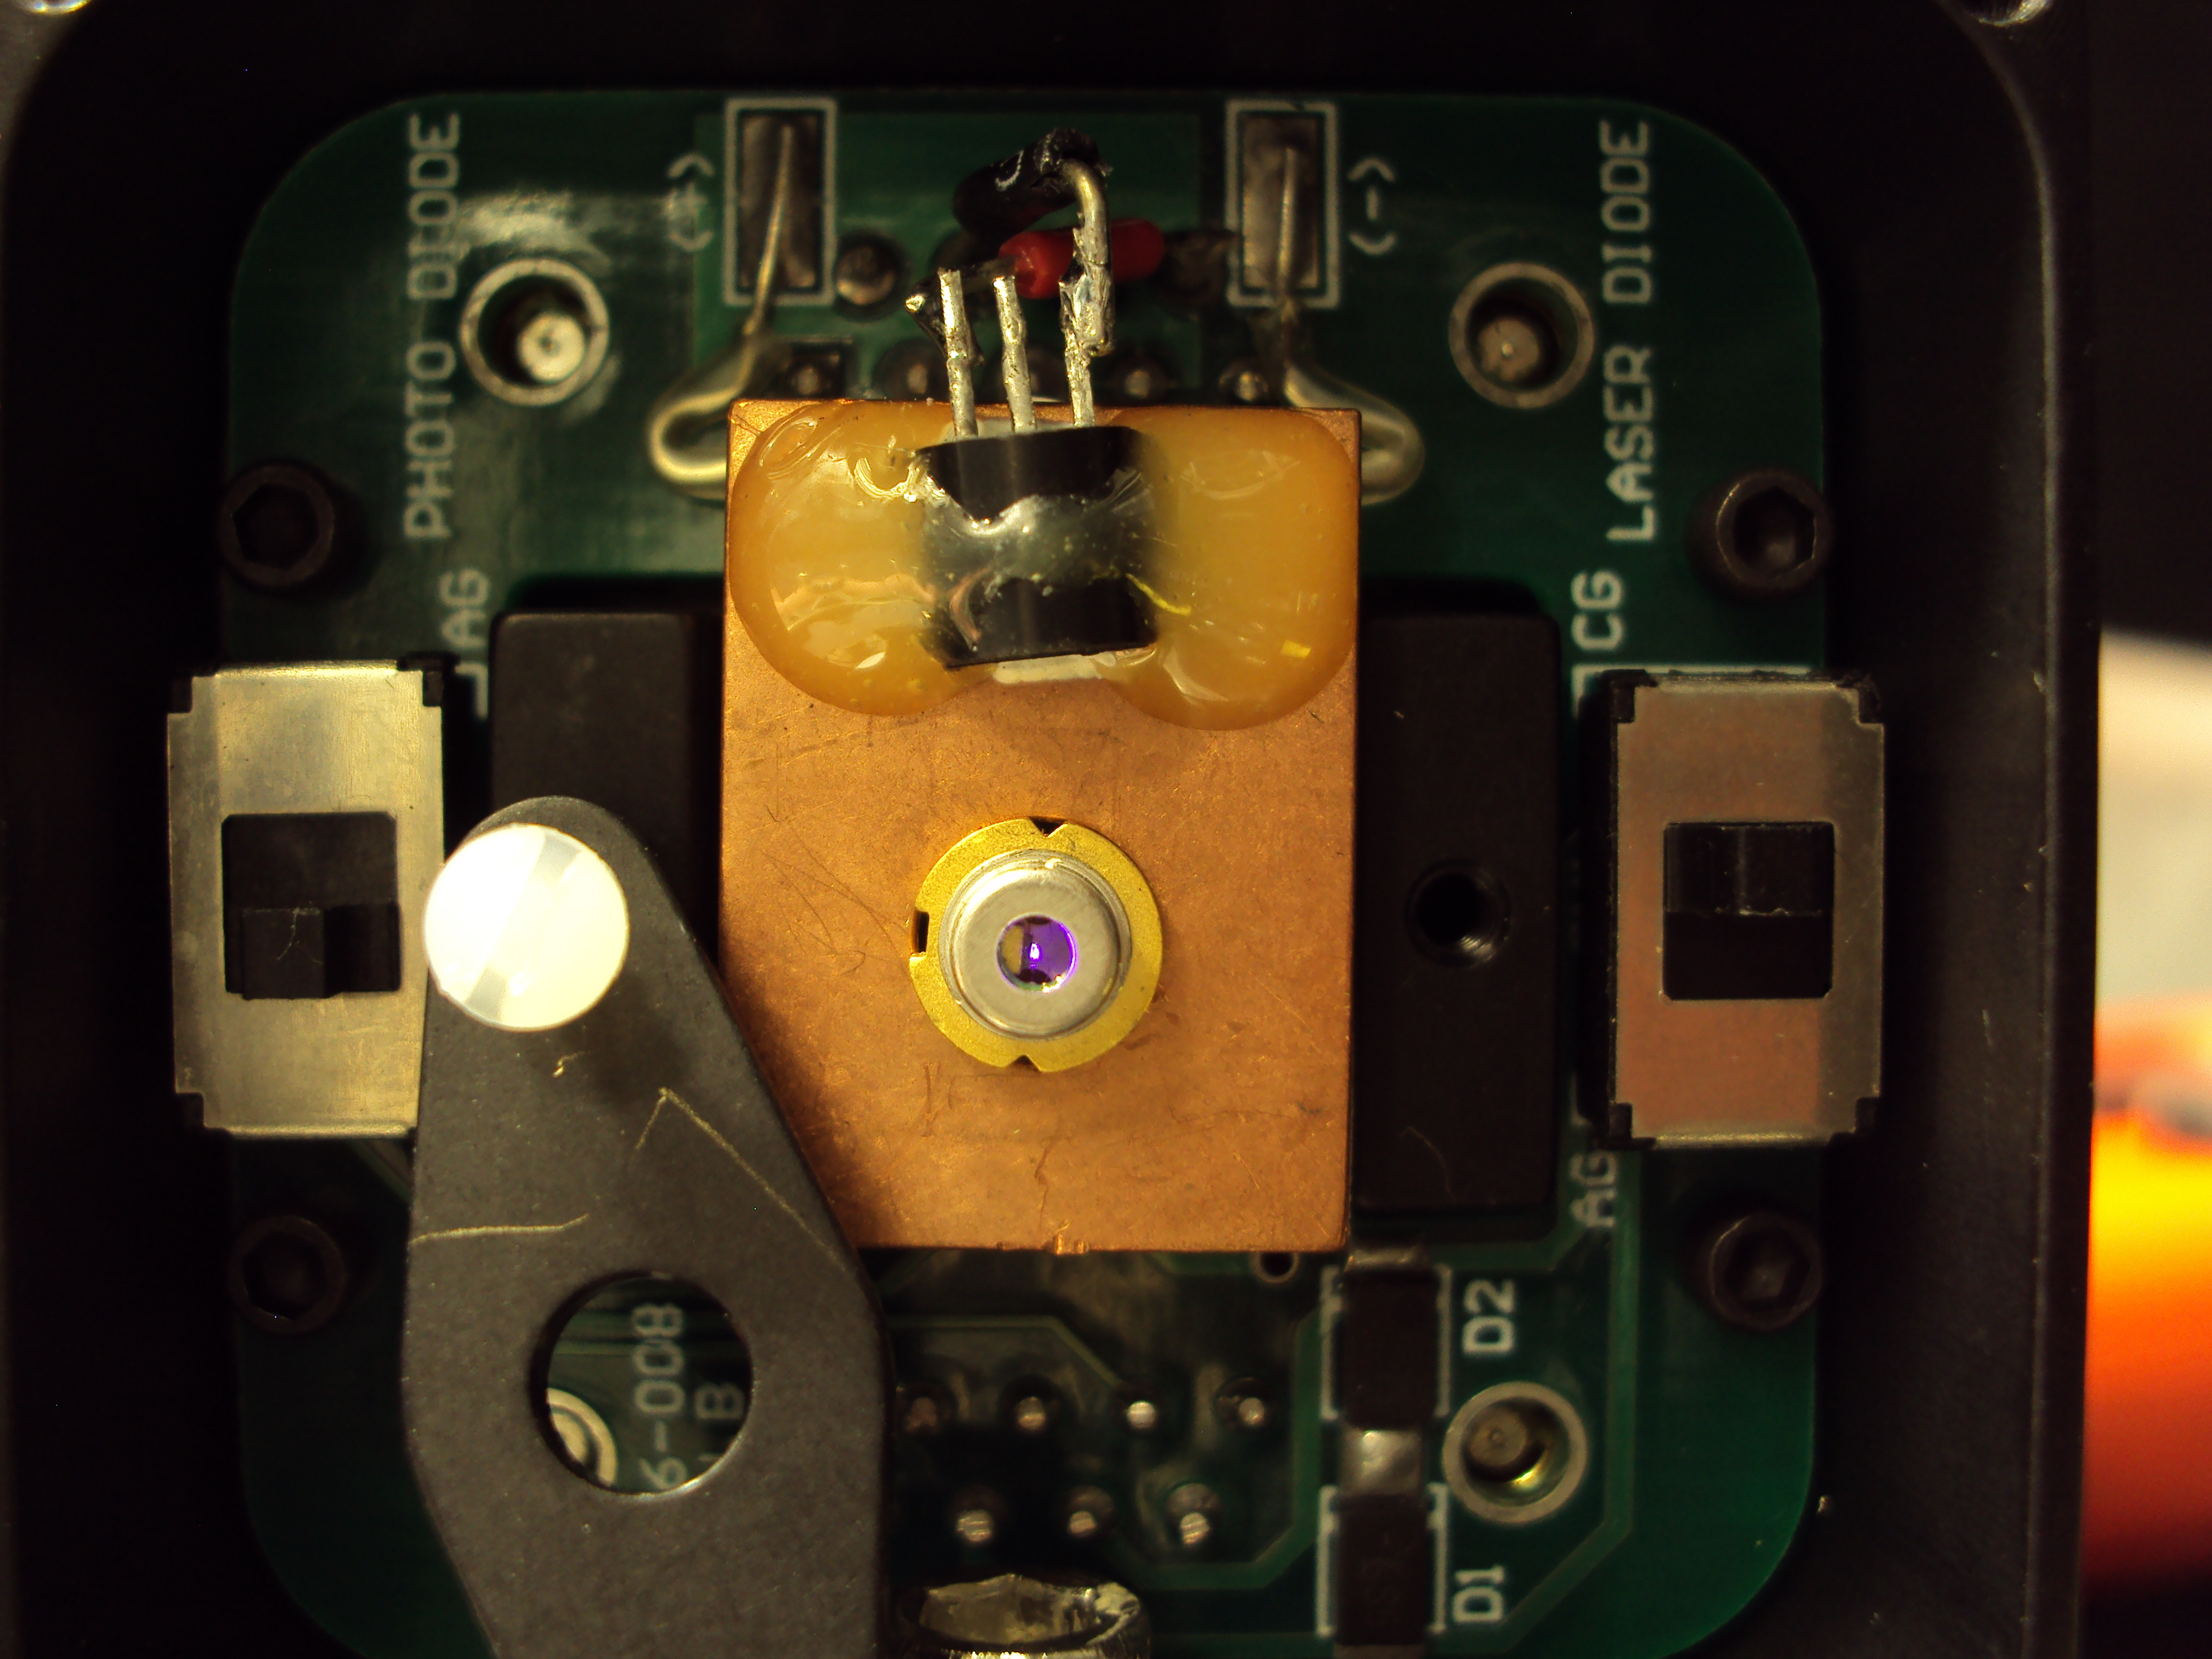
\includegraphics[width=0.95\textwidth]{laser_on_in_housing.JPG}}
\caption[Photograph of Master Laser Diode]{\label{master_laser_interior_photo} The master laser in its housing. We modified the housing to include an additional temperature sensor (the AD592), which can be seen glued to the top of the copper plate.}
\end{figure}
%why did we do the rods? Do I have it in my notes?

\subsection{Master Laser Diodes}
The diodes are single-spatial mode InGaN diodes that are very similar to the diode lasers used in Blu-ray players. 

The diode in the master laser is a Mitsubishi ML320G2, which was wavelength-selected diode by the distributor (i.e. the distributor performed measurements and binned the parts based on their output wavelengths; we then ordered lasers from their 408 nm bin).
As backup diodes, we also bought $\sim 10^1$ diodes on eBay that had been removed from Blu-ray or HD-DVD players and measured their wavelengths in order to bin them ourselves. Some of these diodes were ultimately used in the slave lasers.

We initially tried to build the Master Laser using a non-wavelength-selected Sharp GH04020A2GE low power diode, which we could not stabilize for unknown reasons. We quickly switched to a non-wavelength-selected Sharp GH04P21A2GE diode for the Master laser. However, this laser's free-running wavelength at 25$^\circ$C was far too low. In order to tune this diode to the correct wavelength, we found that we had to maintain the diode at a temperature of $\sim$60$^\circ$C. This resulted in degradation of the diode and loss of power over the course of $\sim 10^2$ days.

\subsection{Grating Spectrometer Wavelength Measurements}

We used a compact grating spectrometer from the Ocean Optics USB2000 series to measure the center frequency of the bare laser diodes. This spectrometer uses a diffraction grating to separate light based on its constituent wavelenghts. Light scattered off the diffraction grating is detected by a CCD array consisting of 2048 pixels that is also enclosed in the spectrometer. The average difference in wavelength between adjacent pixels is $\sim$.061 nm. % This according to /research/octave/ooSpectrumData12Sep/MasterFile.m using the lambdas variable defined in there.

We tried to maximize the resolution and accuracy of our measurements. The center wavelength of the bare diodes changed only a few nanometers over the entire range of possible temperatures and currents. In order to ensure accurate absolute wavelength measurements, we calibrated to a mercury source both before and after looking at the spectra of the various lasers. We feel confident in our calibrations since Mercury conveniently has spectral lines at 405 and 436 nm, which are close to our target wavelength of 407.771 nm. When analyzing the peaks, we fit the measured data to a Gaussian distribution in hopes of squeezing out some sub-pixel level resolution of the peak location. 



We also had a Bristol 521 Wavelength meter, which uses a Michelson-Morley interferometer to measure wavelength. However, for the free-running lasers, we used the spectrometer since the linewidth of the free-running diodes was too large for use with the wavelength meter. 

%diagram of which method to use where? 
The basic 


\subsection{Master Laser Temperature and Current Selection}

The temperature and the current of the laser are two of the main means we have for affecting the wavelength of the Master Laser. Using a grating spectrometer, we measured the center wavelength of the bare laser (no grating installed). 



We have a graph of the temperature and current for all of our lasers. We see that the variation of the center wavelength of the laser is linear to a good approximation over reasonable values of temperature and current.

\begin{figure}
\centering
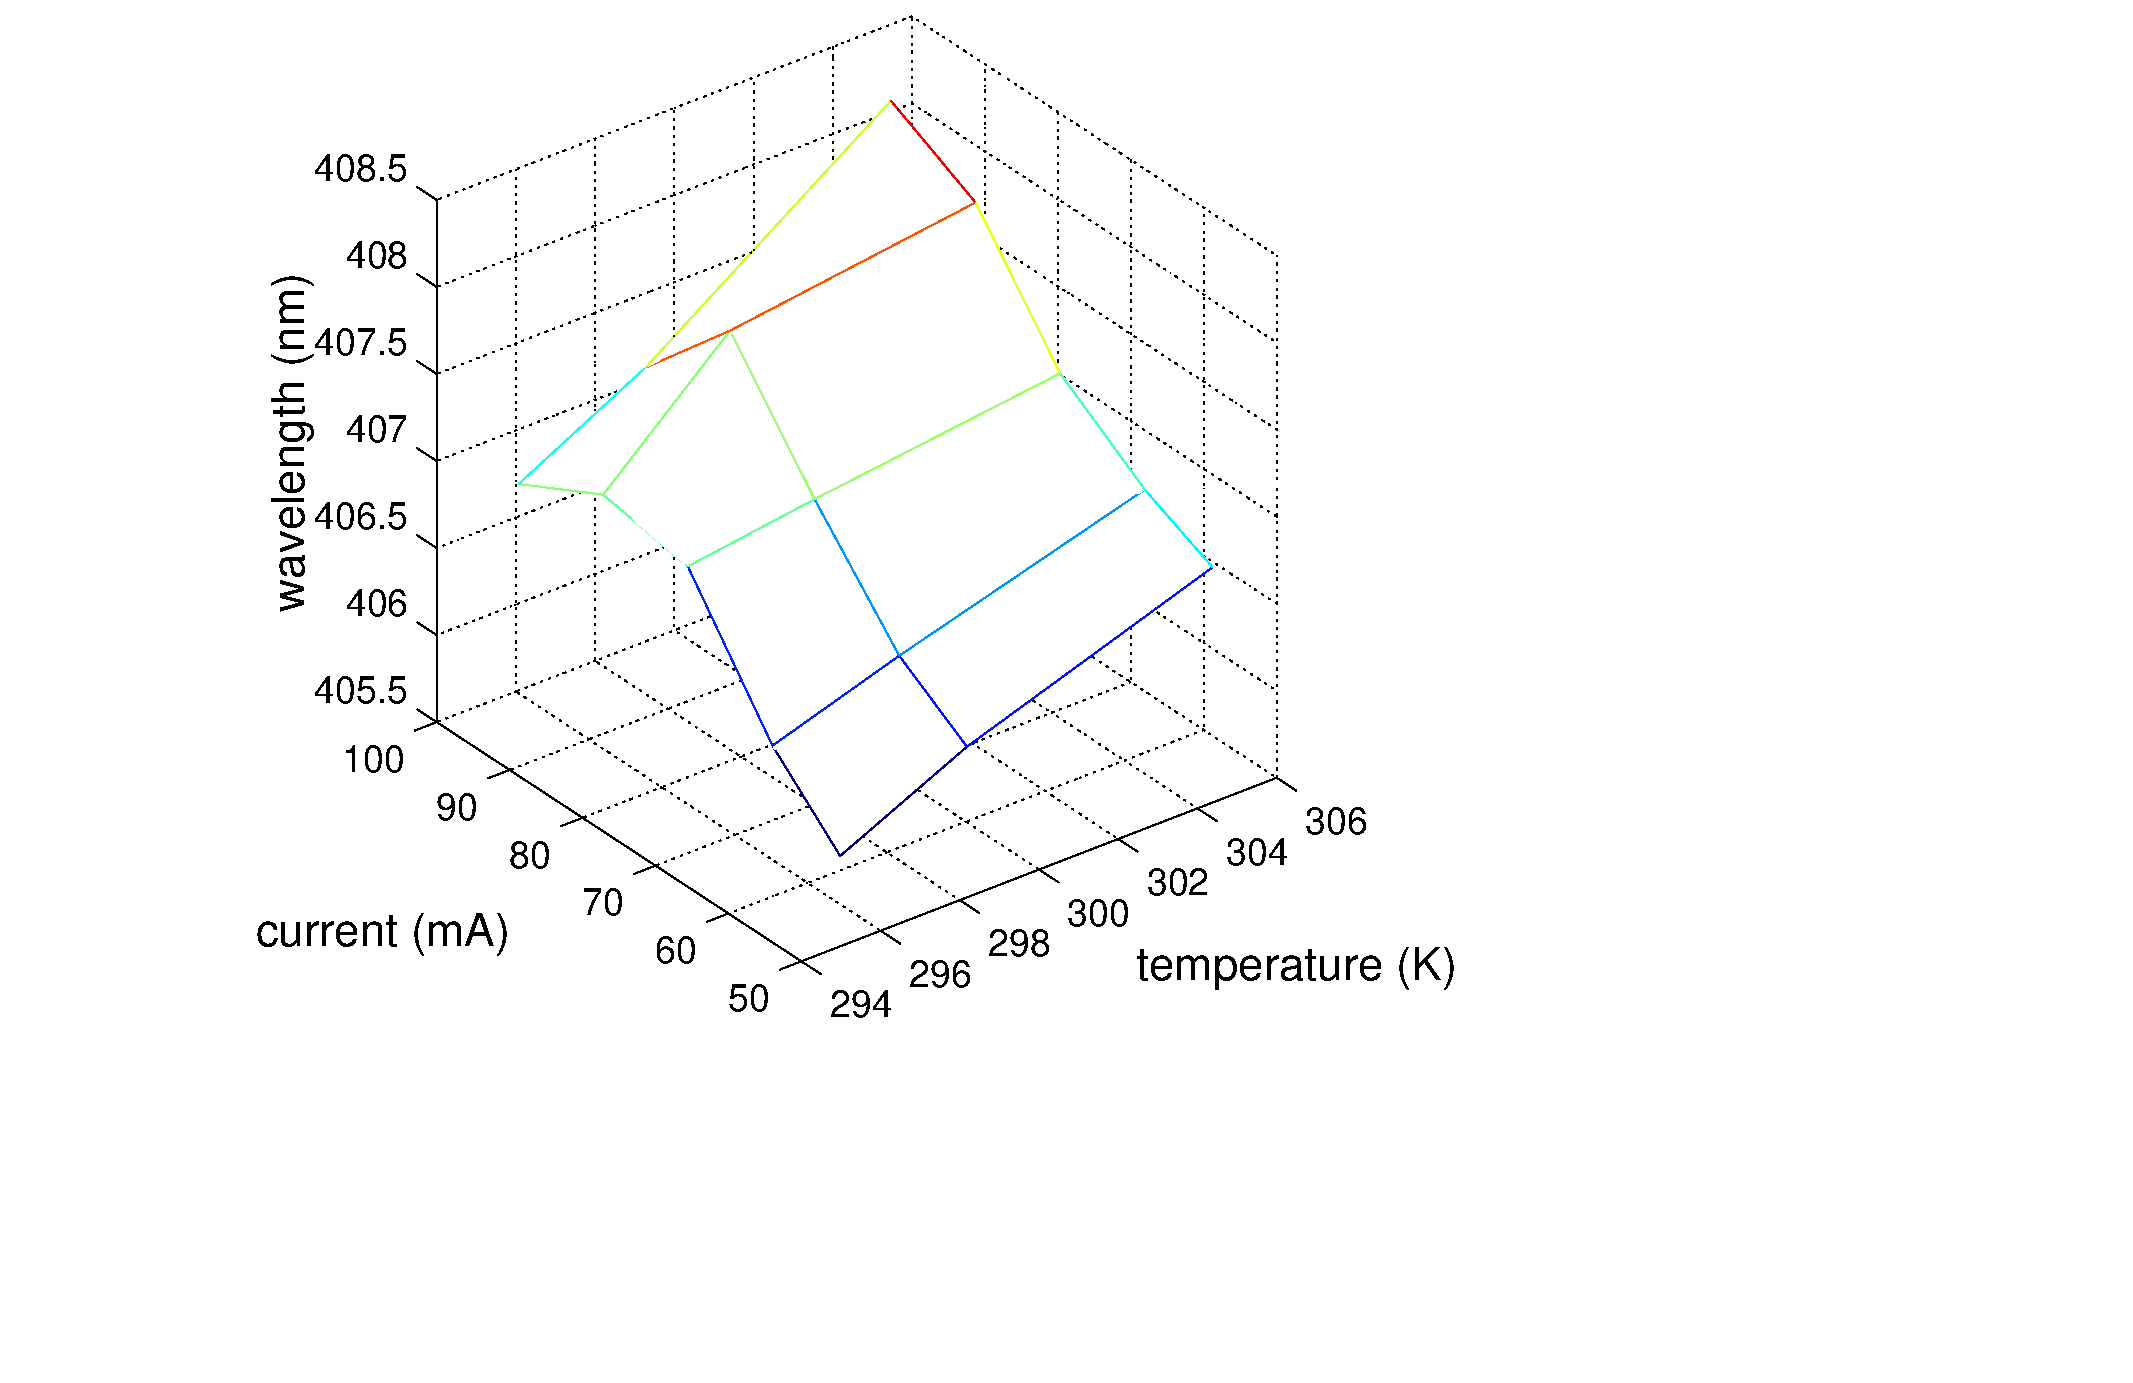
\includegraphics[width=0.7\textwidth]{TVlambda3} 
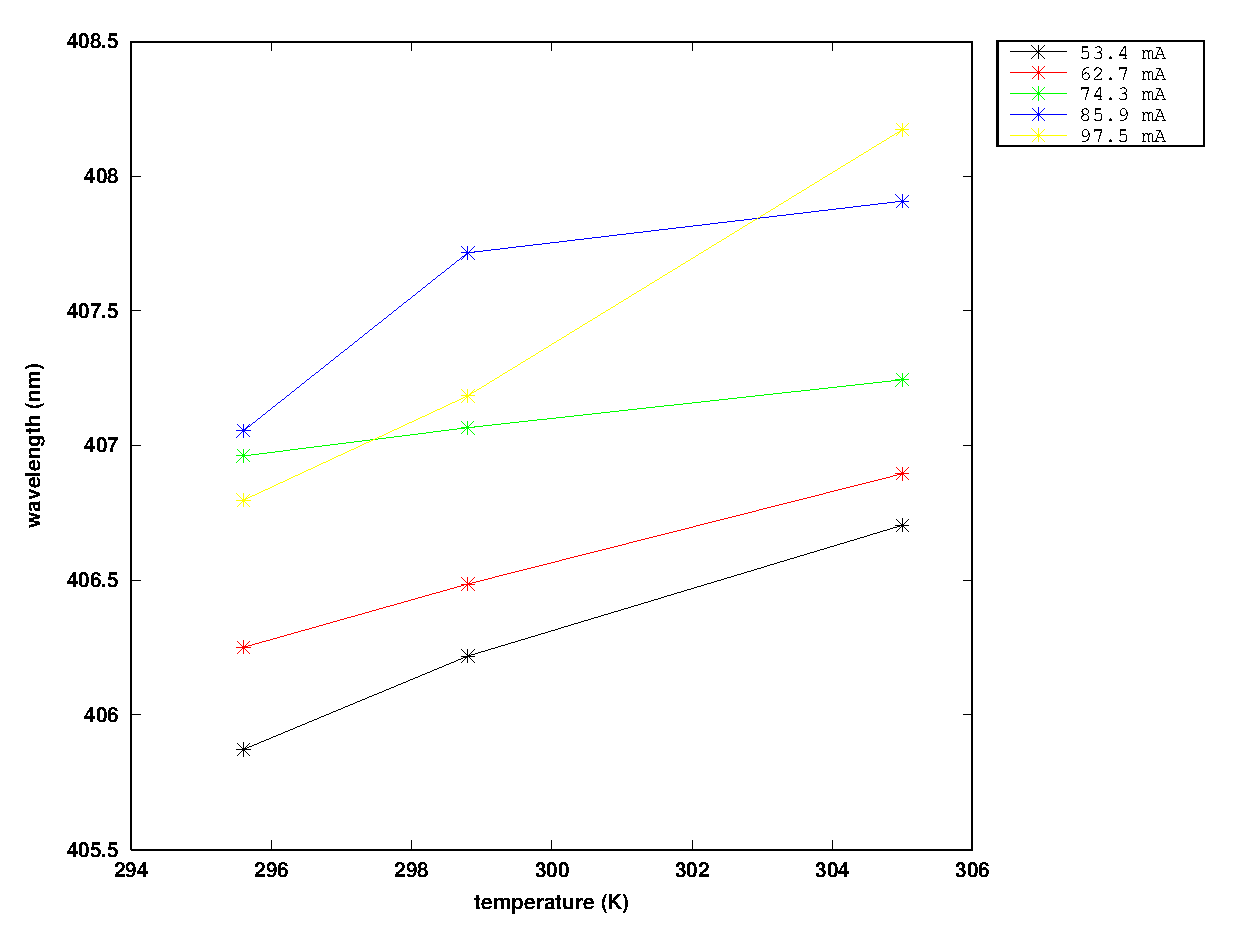
\includegraphics[width=0.7\textwidth]{TVlambda2}
\caption[Graph of Temperatures and Currents]{\label{3dCurrentandTgraph} Representative data of the free-running wavelength of our master laser as a function of nominal current and nominal temperature.}
\end{figure}
%possibly not the master? ehhh. IDK. 

%\footnote{I have no idea what accounts for the variation between diodes}. 

\begin{figure}
\centering
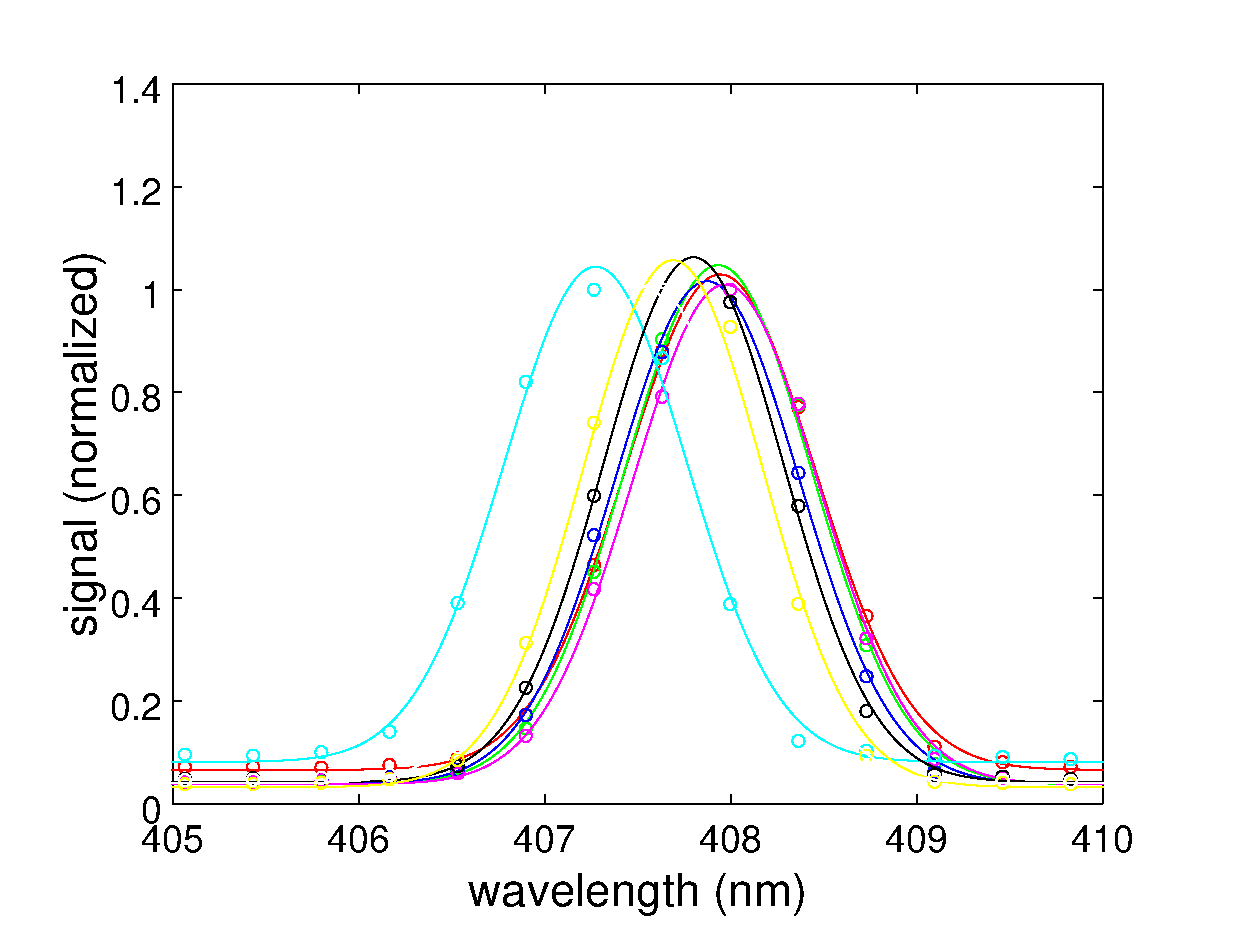
\includegraphics[width=0.95\textwidth]{wavelength_selected} 
\caption[Graph of Temperatures and Currents]{\label{3dCurrentandTgraph} Representative data of the free-running wavelength of our master laser as a function of nominal current and nominal temperature.}
\end{figure}
\begin{figure}
\centering
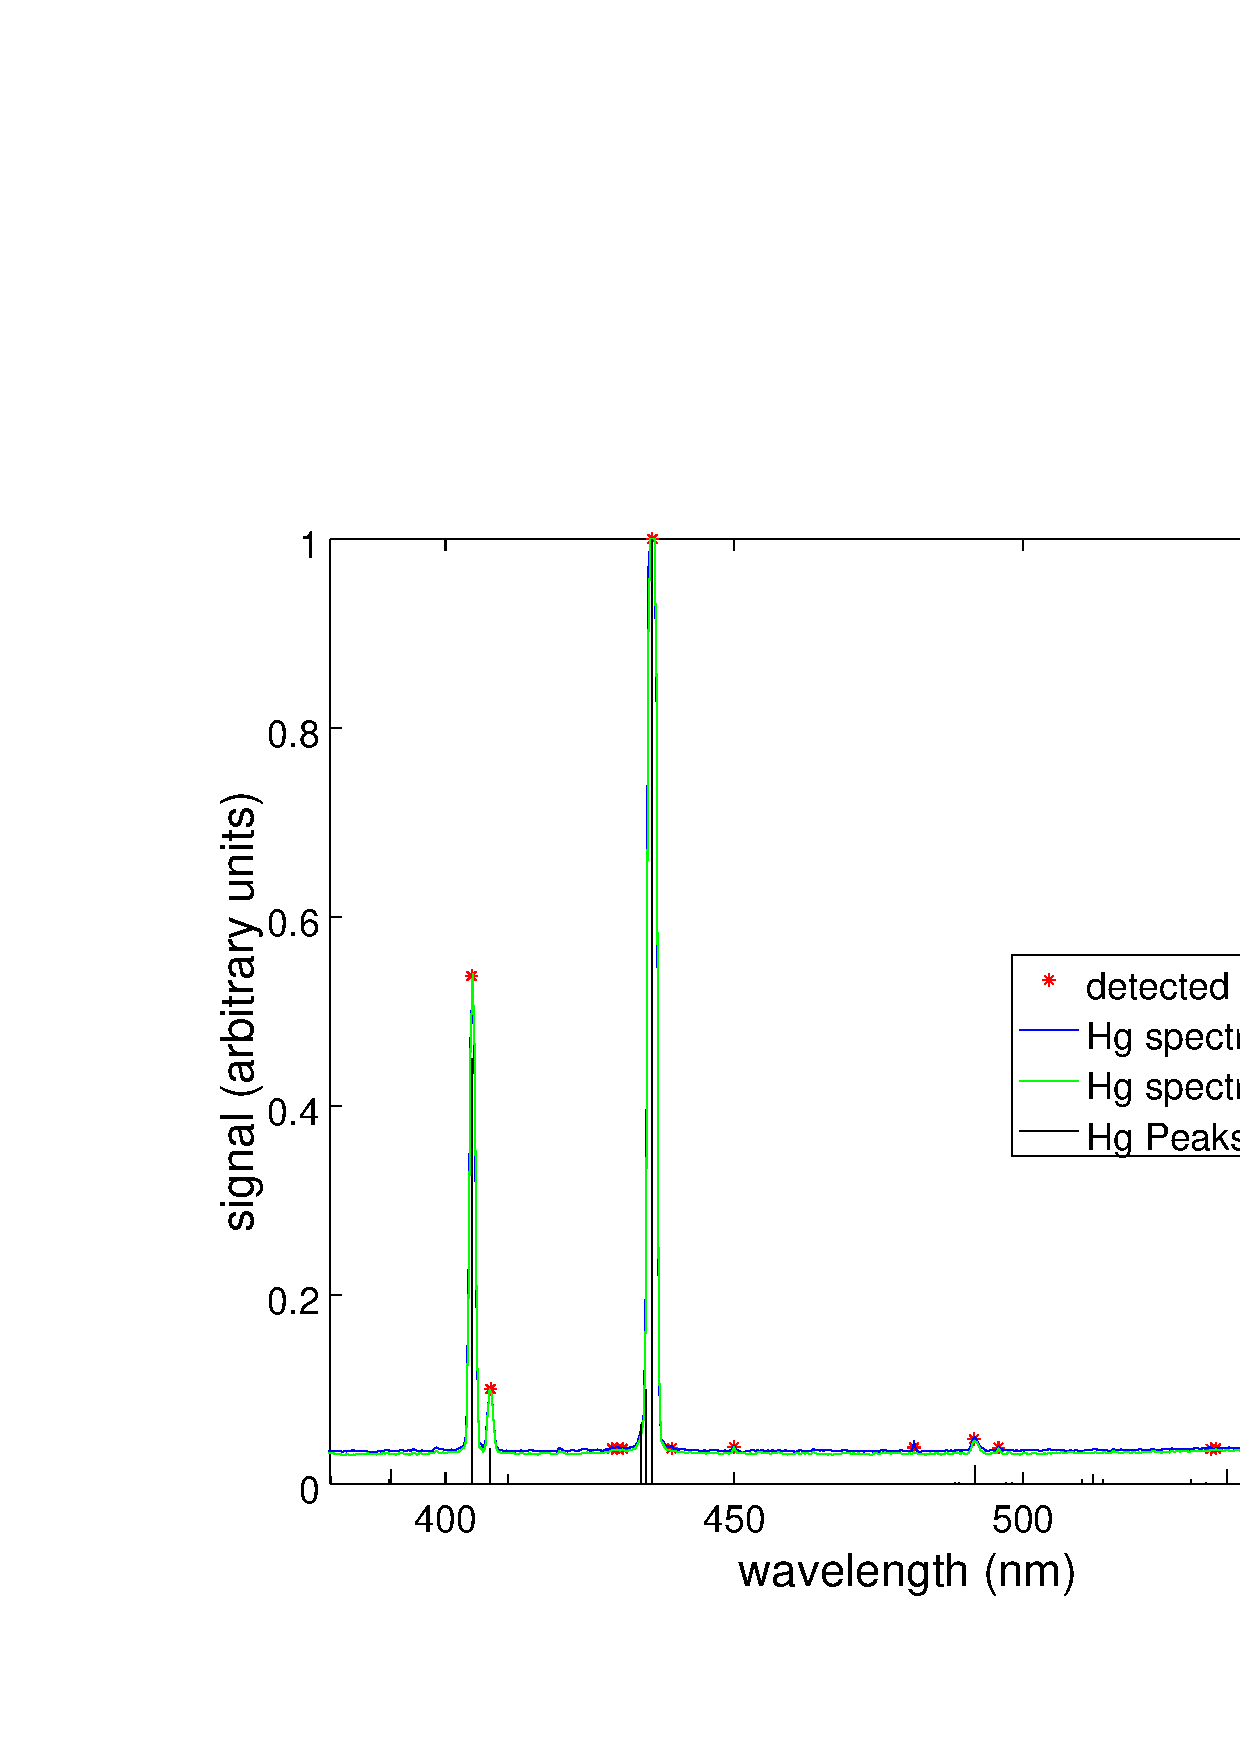
\includegraphics[width=0.95\textwidth]{calibrationData} 
\caption[Graph of Temperatures and Currents]{\label{calibrationData} Data from the calibration using the mercury lamp. We deliberately allowed some of the farther away peaks to saturate in order to improve our signal for the peaks near 408 nm. The black lines represent spectral lines taken from \cite{}}
\end{figure}

\begin{figure}
\centering
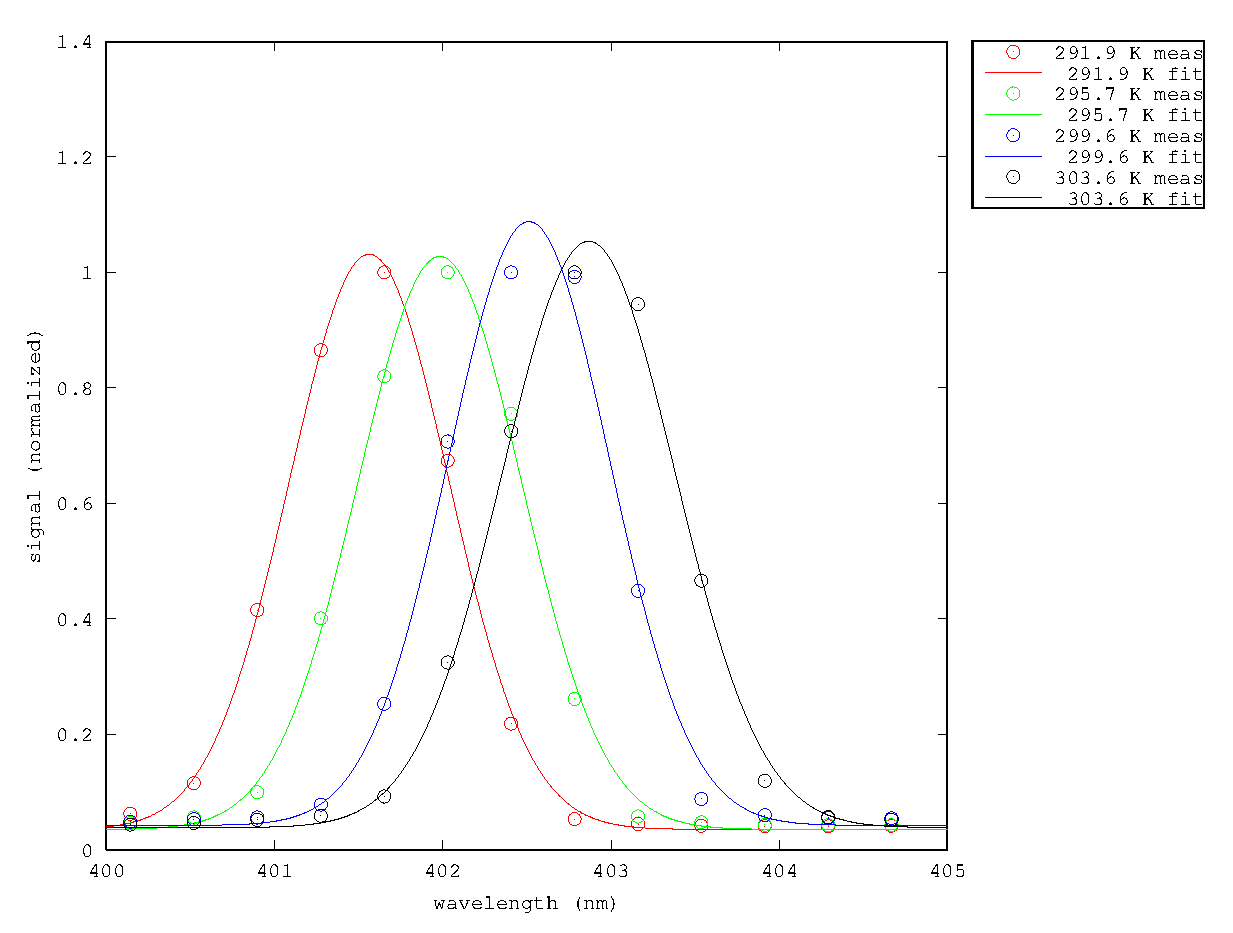
\includegraphics[width=0.95\textwidth]{temperatureFit} 
\caption[Graph of Temperatures and Currents]{\label{3dCurrentandTgraph} Representative data of the free-running wavelength of our master laser as a function of nominal current and nominal temperature.}
\end{figure}

\subsection{Placement of the Grating}

%Some theory here might be worth reviewing. In addition, I did that really great mathematica notebook where I calculated all that stuff. 

%Installation of a diffraction grating allows us to selectively couple light of particular wavelengths back into 

The fundamental process involved in lasing is amplification of light resonant with a particular mode of the laser cavity via stimulated emission. Ideally, we would like to favor a mode within the diode laser corresponding to our desired wavelength. Furthermore, we can additionally favor modes and narrow the linewidth of our laser by adding yet another resonant cavity outside our laser. We thus install an element to selectively couple light at particular wavelengths back into the laser. 

To do this we construct an Extended Cavity for our diode laser (thereby creating an Extended Cavity Diode Laser or ECDL). The extended cavity is formed between the front face of the laser and the diffraction grating that we installed. We must ensure that the diffraction grating is installed such that both the angle and the cavity length match our desired wavelength. To this end, we install the grating on a Thorlabs piezoelectric mount.

The master laser is grating stabilized using an extended cavity formed by a diffraction grating mounted on a piezoelectric mount.  
We installed a 3600 lines/inch diffracting grating (Thorlabs model number GH13-36U) in a custom mount approximately 2 cm from the aperture of collimating lens. The grating is mounted at such an angle that it selectively couples light with a wavelength near 408 nm back into the laser cavity. The resonant space between the diffraction grating and the collimating lens is what the phrase ``extended cavity'' refers to. The additional boundary conditions imposed on the resonant modes of the laser by the external grating result in a narrowing of the laser's linewidth. 
The custom-made grating holder that I fabricated is on display in Figure\,\ref{master_laser_photo}. The motion of the piezoelectric mount is not entirely trivial. The PID controller used to keep the things mounted %did I ever tune this up? 
allows for several gains to be set. The ratio between each of these is strategically calculated to ensure that the output of the PID controller circuitry corresponds to motion on the piezos that allows the favored angle for the diffraction grating to track along with the overall change in length of the cavity. 
 
The diffraction grating is angled so that the 407.771 nm light that we want is directed back into the laser. The condition for this to be the case is 

\begin{equation}
n \lambda = 2 d \cos(\theta),
\end{equation}

Where $d$ is the grating spacing, $n$ is an integer and $\theta$ is the angle of incidence to the grating. 

Furthermore, we would like our cavity's length to increase proportionally with the change in the angle. Thus, from the equilibrium position, we want 

\begin{equation}
\frac{d \lambda}{d k} = \frac{d \lambda}{d k},
\end{equation}

where the LHS represents the derivative of the wavelength favored by the grating angle as a function of the output from the PID controller and the RHS represents the derivative of the wavelength favored by the cavity length as a function of angle. 

%on some level, we need to know what longitudinal order our wavelength was. I mean, it's not that we just move it out one cavity length to change it by a free spectral range. I don't understand why it doesn't always work better with more light coupled back in. Lasers are weird. 

%couldn't we have done much better? I'm not sure. 

\subsection{Calculation of Maximum Safe Intensity}
In order to avoid killing the laser diode, we assumed that the maximum current for which the diode is rated corresponds to the maximum amount of power that can be emerging through the front facet of the laser. We put the maximum recommended current of 25 mA through the laser and measured the output to be \footnote{I need to look up where I did these calculations}. Then we measured the efficiency of the grating by moving the grating so that the light was not reflected into the laser. This way, we could could model the external cavity and deduce what the maximum allowable power coming out of the the cavity corresponded to the maximum power coming out of the laser. The maximum allowable current turned out to be around 100 mA. 

%TODO: look at the peaks of the laser cavity that you did before when Dallin said ``You better make good notes and put that in your thesis''
 
TODO: put in the T and I vs $\lambda$ graphs. 

We installed the diffraction grating on a custom-made mount. 

TODO: figure out what grating you used 

Standard 

%check out ooSpectrumData

%do I have wavelength vs. temperature readings? Yes of course. 
